\apendice{Especificación de Requisitos}

\section{Introducción}
Vamos a analizar profundamente  todo lo referente a los objetivos del proyecto,si las metas ,arcadas en un principio han sido alcanzadas y los requisitos que hemos establecido para guiarnos a lo largo del proyecto.
\section{Objetivos generales}
Desde el comienzo del proyecto se propusieron unos objetivos sobre los cuales construir el proyecto.
\begin{itemize}
\item Como bien vemos en el nombre del proyecto, predicción de apuestas deportivas, este es sin duda la piedra angular del proyecto sobre la que elaborar el resto. Hay que obtener el resultado final de partidos de fútbol, esto lo lograremos utilizando redes neuronales.

\item Una vez tenemos los resultados de los partidos, estos hay que mostrarlos a los usuarios, lo realizaremos utilizando una interfaz sencilla y atractiva, la cual pueda utilizar el usuario,dado que estamos tratando con las apuetsas deportivas se van a mostrar algunas cuotas de las casas de apuestas.

\item Dado que no se puede estar a diario pesando que algoritmos de scraping ejecutar o que datos hay que mostrar es necesario automatizar todo, de esta manera el usuario tendrá toda la información actualizada y no esperar la intervención humana.
\end{itemize}
\section{Catalogo de requisitos}
En este apartado vamos a ver todas las características que posee nuestro proyecto y que se han implementado. Podremos ver todos los requisitos funcionales.

\begin{itemize}
\item \textbf{RF-1: }Se deben obtener todos los datos mediante técnicas de web scraping y almacenarlos en la base de datos.
\begin{itemize}
\item \textbf{RF-1.1: }Se tienen que obtener los resultados de los partidos disputados.

\item \textbf{RF-1.2: }Se debe obtener cada jornada los datos de cada equipo en la clasificación.

\item \textbf{RF-1.3: }Se deben conseguir las cuotas de diferentes casas de apuestas en los partidos de cada jornada.

\item \textbf{RF-1.4: }los datos del web scraping se deben almacenar en la base de datos.

\end{itemize}

\item \textbf{RF-2: }Disponer de una red neuronal capaz de predecir resultados de futuras jornadas.
\begin{itemize}

\item \textbf{RF-2.1: }Hacer un cálculo de las rachas para las instancias de entrada en la red neuronal.

\item \textbf{RF-2.2: }Preprocesar los datos de entrada para acomodarlos a lo que espera la red neuronal.

\item \textbf{RF-2.3: }Realizar el reentrenamiento de la red con los datos de la BBDD.

\item \textbf{RF-2.4: }Realizar la predicción de los partidos de las siguientes jornadas y almacenarla en la base de datos.

\end{itemize}

\item \textbf{RF-3: }Diseño de la página web intuitiva permitiendo una buena interacción con el usuario.

\begin{itemize}
\item \textbf{RF-3.1: }Realizar la administración de Bootstrap.

\item \textbf{RF-3.2: }Se deberá poder observar lo logrado en el global de jornadas previas.

\item \textbf{RF-3.3: }Se deberá poder observar detalladamente cada jornada.

\item \textbf{RF-3.4: }Se podrá observar el pronóstico realizada para la próxima jornada.
\end{itemize}

\end{itemize}

\section{Especificación de requisitos}
En esta sección vamos a apreciar más detalladamente lo referente a los casos de uso.

\subsection{Casos de uso}

En la figura \ref{fig:DiagCasUso}, podemos observar el diagrama de casos de uso del programa, a continuación vamos a ver más detalladamente cada caso de uso. Son tres los actores que podemos encontrar en el diagrama de casos de uso y es que el demonio se encarga de la ejecución automática, pero el administrador si lo desea también puede realizar las diferentes ejecuciones. Por último el usuario únicamente puede visualizar la interfaz.

\begin{figure}
\centering
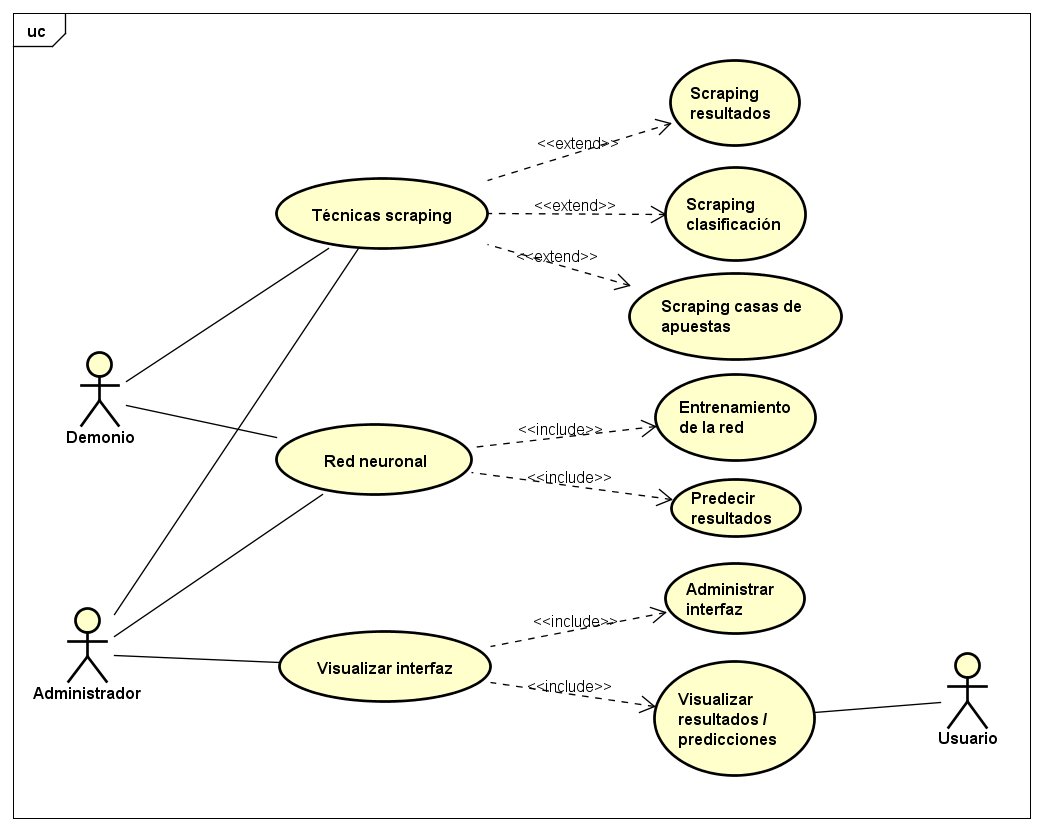
\includegraphics[width=.9\textwidth]{img/diagrama_casos_uso}
\caption{Diagrama completo de los casos de uso.}
\label{fig:DiagCasUso}
\end{figure}

 
\begin{table}
  \begin{center}
   \begin{tabular}{|p{3cm} | p{9cm} |}
    \hline
    Caso de uso & Técnicas scraping\\
    \hline
    Requisitos & RF-1\\
	    & RF-1.1\\
	    & RF-1.2\\
    	& RF-1.3\\
	    & RF-1.4\\
    \hline
    Descripción & El sistema obtiene todos los datos necesarios para poder utilizar la red neuronal y para poner en la interfaz.\\
    \hline
    Precondiciones & Los datos no han sido recopilados previamente.\\
    \hline
    Acciones & 1. El administrador ejecuta los algoritmos de scraping desde Drupal, o bien espera la ejecución automática del demonio. \\
    &2. La aplicación realiza la ejecución. \\
    &\hspace{1em} 2.1 Se recopilan los datos en la base de datos.\\
    &\hspace{1em} 2.2 Se actualiza la interfaz web.\\
    \hline
    Postcondiciones & Ninguna \\
    \hline
    Excepciones & Si se intentan introducir los datos de nuevo se produce un error en el sistema. \\
    \hline
    Importancia & Alta \\
    \hline
   \end{tabular}
   \caption{Caso de uso ``Técnicas scraping''.}
   \label{tabla:casoUso1}
  \end{center}
 \end{table} 
 
 \begin{table}
  \begin{center}
   \begin{tabular}{|p{3cm} | p{9cm} |}
    \hline
    Caso de uso & Red neuronal\\
    \hline
    Requisitos & RF-2\\
	    & RF-2.1\\
	    & RF-2.2\\
    	& RF-2.3\\
    	& RF-2.4\\
    \hline
    Descripción & El demonio o el administrador lanza la ejecución del algoritmo de backpropagation sobre la red neuronal para conseguir el pronóstico de los partidos.\\
    \hline
    Precondiciones &Los datos han sido recopilados previamente.\\
    \hline
    Acciones & 1. Se realiza el cálculo de las rachas de los equipos. \\
    &2. La aplicación realiza el preprocesamiento previo a la entrada de las instancias en la red neuronal.\\
    &3. Se cargan los datos en la red neuronal y se realiza el entrenamiento.\\
    &4. Se lleva a cabo el test y se almacenan los datos obtenidos en la base de datos.\\
    \hline
    Postcondiciones & Ninguna \\
    \hline
    Excepciones & Si ya se ha realizado ya la carga de datos de los pronósticos en la base de datos no se lleva a cabo de nuevo. \\
    \hline
    Importancia & Alta \\
    \hline
   \end{tabular}
   \caption{Caso de uso ``Red neuronal''.}
   \label{tabla:casoUso2}
  \end{center}
 \end{table} 
 
\begin{table}
  \begin{center}
   \begin{tabular}{|p{3cm} | p{9cm} |}
    \hline
    Caso de uso & Visualizar interfaz\\
    \hline
    Requisitos & RF-3\\
	    & RF-3.1\\
	    & RF-3.2\\
    	& RF-3.3\\
    	& RF-3.4\\
    \hline
    Descripción & El sitio web recoge los datos proporcionados por la red neuronal y el algoritmo de scraping de las casas de apuestas.\\
    \hline
    Precondiciones &Los datos han sido recopilados previamente.\\
    &Se han llevado a cabo el correspondiente cálculo de las jornadas.\\
    \hline
    Acciones & 1. Se podrá observar un resumen global con los valores de cada jornada. \\
    &2. De manera individual cada jornada se puede observar más detalladamente.\\
    &3. El pronóstico de la siguiente jornada estará disponible para oriental al usuario.\\
    &4. Se podrá realizar una gestión de la interfaz visual, así como modificar textos o tablas.\\
    \hline
    Postcondiciones & Ninguna \\
    \hline
    Excepciones & Ninguna\\
    \hline
    Importancia & Media \\
    \hline
   \end{tabular}
   \caption{Caso de uso ``Visualizar interfaz''.}
   \label{tabla:casoUso3}
  \end{center}
 \end{table} 
 
 \begin{table}
  \begin{center}
   \begin{tabular}{|p{3cm} | p{9cm} |}
    \hline
    Caso de uso & Scraping resultados\\
    \hline
    Requisitos & RF-1.1\\
    & RF-1.4\\
    \hline
    Descripción & Extraemos los datos de los partidos de fútbol ya disputados mediante web scraping.\\
    \hline
    Precondiciones &Los partidos deben haberse disputado.\\
    \hline
    Acciones & 1. Se accede uno a uno a cada partido mediante la url. \\
    &2. Se extraen los datos de ambos equipos.\\
    &3. Se almacenan los datos en la base de datos.\\
    \hline
    Postcondiciones & Ninguna \\
    \hline
    Excepciones & No se recogen si se han recogido previamente.\\
    \hline
    Importancia & Alta \\
    \hline
   \end{tabular}
   \caption{Caso de uso ``Scraping resultados''.}
   \label{tabla:casoUso1.1}
  \end{center}
 \end{table} 
 
\begin{table}
  \begin{center}
   \begin{tabular}{|p{3cm} | p{9cm} |}
    \hline
    Caso de uso & Scraping clasificación\\
    \hline
    Requisitos & RF-1.2\\
    & RF-1.4\\
    \hline
    Descripción & Extraemos los datos de la clasificación para cada uno de los equipos mediante web scraping.\\
    \hline
    Precondiciones &Los partidos deben haberse disputado.\\
    \hline
  	Acciones & 1. Se accede a la clasificación donde se encuentran todos los datos de los equipos. \\
    &2. Se extraen los datos de la clasificación de cada equipo.\\
    &3. Se almacenan los datos en la base de datos.\\
    \hline
    Postcondiciones & Ninguna \\
    \hline
    Excepciones & No se recogen si se han recogido previamente.\\
    \hline
    Importancia & Alta \\
    \hline
   \end{tabular}
   \caption{Caso de uso ``Scraping clasifiación''.}
   \label{tabla:casoUso1.2}
  \end{center}
 \end{table} 

\begin{table}
  \begin{center}
   \begin{tabular}{|p{3cm} | p{9cm} |}
    \hline
    Caso de uso & Scraping casas de apuestas\\
    \hline
    Requisitos & RF-1.3\\
    & RF-1.4\\
    \hline
    Descripción & Extraemos los datos de la clasificación para cada uno de los equipos mediante web scraping.\\
    \hline
    Precondiciones &Los partidos no deben haberse disputado.\\
    &La recopilación de datos hay que hacerla en la fecha más cercana posible para tener los últimos datos.\\
    \hline
  	Acciones & 1. Accedemos uno a uno a los partidos de la jornada que está por disputar. \\
    &2. Se extraen las cuotas de las cuatro casas de apuestas que se encuentran en la web.\\
    &3. Se almacenan los datos en la base de datos.\\
    \hline
    Postcondiciones & Ninguna \\
    \hline
    Excepciones & No se recogen si se han recogido previamente.\\
    \hline
    Importancia & Baja \\
    \hline
   \end{tabular}
   \caption{Caso de uso ``Scraping casas de apuestas''.}
   \label{tabla:casoUso1.4}
  \end{center}
 \end{table} 


\begin{table}
  \begin{center}
   \begin{tabular}{|p{3cm} | p{9cm} |}
    \hline
    Caso de uso & Entrenamiento de la red\\
    \hline
    Requisitos & RF-2.1\\
    	& RF-2.2\\
	    & RF-2.3\\
    \hline
    Descripción & Obtenemos los datos de la BBDD , generamos las instancias y preprocesamos los datos antes de introducirlos a la red neuronal, finalmente se introducen para el entrenamiento.\\
    \hline
    Precondiciones &Los datos de partidos y la clasificación deben estar en la BBDD\\
    &Se debe haber hecho el cálculo de las rachas.\\
    \hline
  	Acciones & 1. Accedemos a la BBDD y extraemos los datos necesarios. \\
    &2. Generamos las instancias.\\
    &3. Preprocesamos las instancias.\\
	&4. Introducimos los datos en la red neuronal.\\
    \hline
    Postcondiciones & Llevar acabo la predicción. \\
    \hline
    Excepciones & Ninguna.\\
    \hline
    Importancia & Alta\\
    \hline
   \end{tabular}
   \caption{Caso de uso ``Entrenamiento de la red''.}
   \label{tabla:casoUso2.1}
  \end{center}
 \end{table} 
 

\begin{table}
  \begin{center}
   \begin{tabular}{|p{3cm} | p{9cm} |}
    \hline
    Caso de uso & Predecir resultados\\
    \hline
    Requisitos & RF-2.4\\
	    & RF-1.4\\
    \hline
    Descripción & Obtenemos los datos de la BBDD , generamos las instancias y preprocesamos los datos antes de introducirlos a la red neuronal, finalmente se introducen para el entrenamiento.\\
    \hline
    Precondiciones &Tener la red neuronal entrenada.\\
    \hline
  	Acciones & 1. Realizamos la predicción tres veces y nos quedamos con la media.\\
    &2. Almacenamos los datos obtenidos en la base de datos.\\
    \hline
    Postcondiciones & Ninguna. \\
    \hline
    Excepciones & Si se han almacenado los datos previamente no se vuelve a almacenar.\\
    \hline
    Importancia & Alta\\
    \hline
   \end{tabular}
   \caption{Caso de uso ``Predecir resultados''.}
   \label{tabla:casoUso2.2}
  \end{center}
 \end{table} 
 
 \begin{table}
  \begin{center}
   \begin{tabular}{|p{3cm} | p{9cm} |}
    \hline
    Caso de uso & Administrar interfaz\\
    \hline
    Requisitos & RF-3.1\\
    \hline
    Descripción & El administrador puede realizar diferentes modificaciones respecto a la interfaz, utilizando las herramientas que Drupal proporciona y realizando cambios en los scripts.\\
    \hline
    Precondiciones &Tener permisos de administrador en Drupal.\\
    \hline
  	Acciones & 1. Modificar temas, módulos o bloques.\\
    &2. Se pueden editar los scripts.\\
    \hline
    Postcondiciones & Ninguna. \\
    \hline
    Excepciones & Ninguna.\\
    \hline
    Importancia & Media\\
    \hline
   \end{tabular}
   \caption{Caso de uso ``Administrar interfaz''.}
   \label{tabla:casoUso3.1}
  \end{center}
 \end{table} 
 
  \begin{table}
  \begin{center}
   \begin{tabular}{|p{3cm} | p{9cm} |}
    \hline
    Caso de uso & Visualizar resultados/predicciones\\
    \hline
    Requisitos & RF-3.2\\
    & RF-3.3\\
    & RF-3.4\\
    \hline
    Descripción & El usuario puede observar aquellos datos que le resulten de interés como lo referente a jornadas pasadas y el pronóstico de la próxima jornada.\\
    \hline
    Precondiciones &Datos presentes en la base de datos.\\
    			&Se ha debido realizar las ejecuciones correspondientes del algoritmo de backpropagation.\\
    \hline
  	Acciones & 1. Visualizar el balance global de todas las jornadas.\\
    &2. Visualizar el balance detallado de cada jornada.\\
    &3. Visualizar la predicción de la próxima jornada.\\
    \hline
    Postcondiciones & Ninguna. \\
    \hline
    Excepciones & Ninguna.\\
    \hline
    Importancia & Media\\
    \hline
   \end{tabular}
   \caption{Caso de uso ``Visualizar resultados/predicciones''.}
   \label{tabla:casoUso3.2}
  \end{center}
 \end{table}